%  !TeX  root  =  user_guide.tex 

%\section{Interpolation Plugin}
\section{Extension Interpolation}

% when the revision of a section has been finalized, 
% comment out the following line:
%\updatedisclaimer

%The Interplation plugin can be used to generate a TIN or IDW interpolation of a 
%point vector layer. It is very simple to handle and provides an intiuitive graphical 
%user interface for creating interpolated raster layers (See Figure \ref{fig:interpolation_dialog}).
%The plugin requires the following parameters to be specified before running:
L'extension Interpolation permet de générer une interpolation TIN ou IDW 
depuis une couche vectorielle de points. Cette extension est très simple à 
manipuler et fournit à l'utilisateur une interface graphique intuitive pour la
création de couches matricielles interpolées (voir la Figure \ref{fig:interpolation_dialog}).
Avant son exécution, l'extension nécessite les réglages suivants:

%\begin{itemize}
%\item[Input vector layer :] Specify the input point vector layer(s) from a list of loaded
%point layers. If several layers are specified, then data from all layers is used for
%interpolation. Note: It is possible to insert lines or polygons as constraints for the
%triangulation, by specifying either ``structure lines'' or ``break lines'' in the
%\dropmenuopt{Type} dropdown menu.
%\item[Interpolation attribute :] Select attribute column to be used for interpolation or 
%enable the \checkbox{Use Z-Coordinate} checkbox to use the layers stored Z values.
%\item[Interpolation Method :] Select interpolation method. This can be either \selectstring{Triangulated Irregular 
%Network (TIN)}{\ldots} or \selectstring{Inverse Distance Weighted (IDW)}{\ldots}.
%\item[Number of columns/rows :] Specify the number row and colums for the output raster file.
%\item[Output file :] Specify a name for the output raster file.
%\end{itemize}
\begin{description}
\item[Couches vecteur :] Spécifier une (ou plusieurs) couche 
vectorielle de points parmi la liste de couches vectorielles de points 
chargées. Si plusieurs couches sont sélectionnées, alors l'ensemble des 
données de toutes les couches est utilisé pour l'interpolation. 
Note: il est possible d'insérer des lignes ou des polygones comme contrainte 
pour la triangulation en spécifiant ``lignes de structure'' ou ``break lines'' 
dans la liste déroulante du sous-menu \dropmenuopt{Type}.
%===> 'break lines' non traduit dans l'interface utilisateur JRM: c'est corrigé pour la version 1.5 mais effectviement pour la 1.3 on laisse la vo
\item[Attribut d'interpolation :] Sélectionner une colonne 
attributaire à utiliser pour l'interpolation ou cocher la case 
\checkbox{Utiliser les coordonnées Z pour l'interpolation} afin d'utiliser une
couche contenant des valeurs Z.
\item[Méthode d'interpolation :] Sélectionner une méthode 
d'interpolation. Cela peut être\\ \selectstring{Interpolation Triangulaire (TIN)}{\ldots} 
ou\\ \selectstring{Pondération par Distance Inverse (IDW)}{\ldots}.
\item[Nombre de colonnes/cellules :] Définir le nombre de colonnes et 
de lignes du raster de sortie.
\item[Fichier de sortie :] Attribuer un nom au fichier raster de 
sortie.
\end{description}

%\begin{figure}[ht]
%   \begin{center}
%   \caption{Interpolation Plugin \nixcaption}\label{fig:interpolation_dialog}\smallskip
%   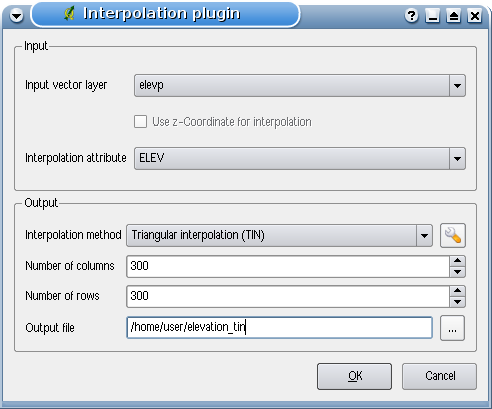
\includegraphics[clip=true, width=9cm]{interpolate_dialog}
%\end{center}  
%\end{figure}
\begin{figure}[ht]
   \begin{center}
   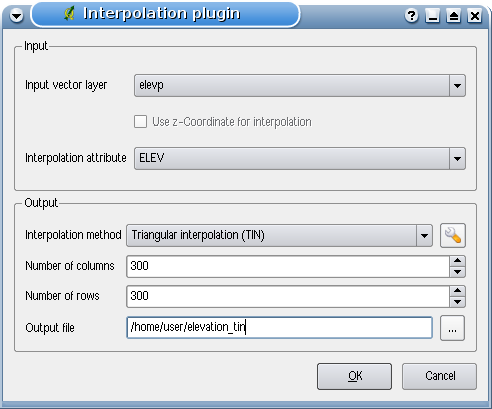
\includegraphics[clip=true, width=9cm]{interpolate_dialog}
   \caption{L'extension Interpolation \nixcaption}\label{fig:interpolation_dialog}
\end{center}  
\end{figure}

%\minisec{Using the plugin}\label{interpolation_usage}
\minisec{Mettre en oeuvre l'extension}\label{interpolation_usage}

%\begin{enumerate}
%  \item Start QGIS and load an point vector layer (e.g., \filename{elevp.csv}). 
%  \item Load the Interpolation plugin in the Plugin Manager (see Section 
%  \ref{sec:load_core_plugin}) and click on the \toolbtntwo{interpolation}{Interpolation} 
%  icon which appears in the QGIS toolbar menu. The Interpolation plugin dialog appears as 
%  shown in Figure \ref{fig:interpolation_dialog}.
%  \item Select an input layer (e.g., \selectstring{elevp}{\ldots}) and column (e.g. \filename{ELEV}) for 
%  interpolation.
%  \item Select an interpolation method (e.g. \selectstring{Triangular interpolation}{\ldots}), and specify 
%  the number of rows and columns (e.g. 3663 cols and 1964 rows (this is equivalent to a 1000 meter pixel resolution))
%  as well as the raster output filename (e.g., \filename{elevation\_tin}).
%  \item Click \button{Ok}.
%  \item For the current example, double click \filename{elevation\_tin} in the layer list to open the Raster Layer Properties 
%  dialog and select \selectstring{Pseudocolor}{\ldots} as Color Map in the \tab{Symbology} tab. Or you 
%  can define a new color table as described in Section \ref{label_rasterprop}.
%\end{enumerate}
\begin{enumerate}
  \item Lancez QGIS et chargez une couche vectorielle de points (par 
  exemple, \filename{elevp.csv}). 
  \item Activez l'extension Interpolation via le Gestionnaire d'Extensions 
  (voir la Section \ref{sec:load_core_plugin}) puis appuyez sur l'icône
  \toolbtntwo{interpolation}{Interpolation} qui apparaît alors dans la barre 
  d'outils QGIS. La boîte de dialogue de l'extension Interpolation s'ouvre 
  comme montrée dans la Figure \ref{fig:interpolation_dialog}.
  \item Dans le bloc Saisie, sélectionnez une couche vectorielle de départ 
  (par exemple,\\ \selectstring{elevp}{\ldots}) ainsi qu'une colonne 
  attributaire pour l'interpolation (par exemple, \filename{ELEV}).
  \item Dans le bloc Rendu, sélectionnez une méthode d'interpolation 
  (par exemple,\\ \selectstring{Interpolation Triangulaire}{\ldots}), puis 
  définissez le nombre de colonnes et de cellules (par exemple, \numprint{3663} colonnes 
  et \numprint{1964} lignes (ce qui équivaut à une résolution de \numprint{1000} mètres par 
  pixels)) ainsi qu'un nom pour le fichier raster de sortie
  (par exemple, \filename{elevation\_tin}).
  \item Appuyez sur \button{Ok}.
  \item Pour cet exemple, double cliquez sur \filename{elevation\_tin} dans la
  liste des couches pour ouvrir la fenêtre de propriétés de la couche raster 
  et sélectionnez \selectstring{Pseudocouleur}{\ldots} comme couleur de la 
  carte dans l'onglet \tab{Symbologie}. Vous pouvez également définir une 
  nouvelle table de couleurs comme décrite dans la Section \ref{label_rasterprop}.
\end{enumerate}

%In Figure \ref{fig:interpolation_idw} you see the IDW interpolation result with a 366 cols x 196 rows (10 km) 
%resolution for the \filename{elevp.csv} data visualized using the Pseudocolor color table. The processing 
%only takes a few minutes, and covers the northern part of Alaska.
Dans la Figure \ref{fig:interpolation_idw} vous pouvez voir le résultat d'une
interpolation IDW avec une résolution de 366 colonnes x 196 lignes (soit 
10 km) pour les données du fichier \filename{elevp.csv}, affichées en utilisant 
une table de coloration en pseudocouleurs. Le traitement ne prend que quelques 
minutes et couvre la partie nord de l'Alaska.

%\begin{figure}[ht]
%   \begin{center}
%   \caption{Interpolation of elevp data using IDW method \nixcaption}\label{fig:interpolation_idw}\smallskip
%   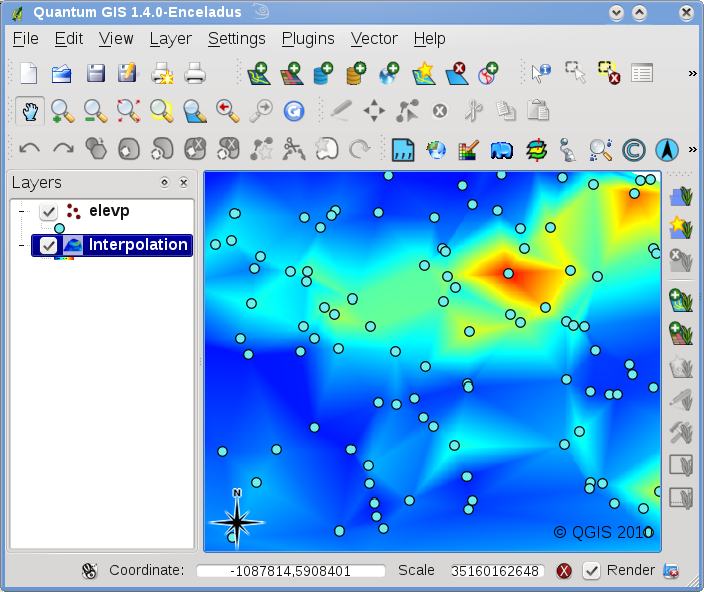
\includegraphics[clip=true, width=10cm]{interpolate_idw}
%\end{center}  
%\end{figure}
\begin{figure}[ht]
   \begin{center}
   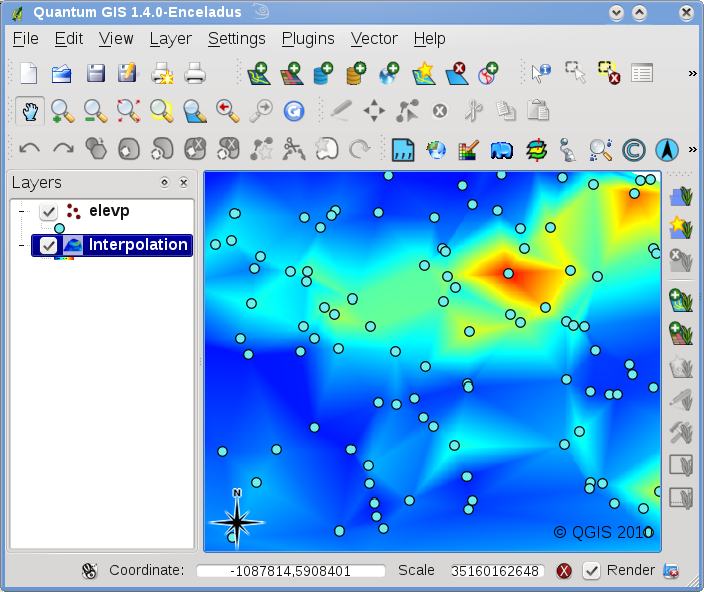
\includegraphics[clip=true, width=10cm]{interpolate_idw}
   \caption{Interpolation IDW sur le fichier elevp \nixcaption}\label{fig:interpolation_idw}
\end{center}  
\end{figure}